\documentclass[a4paper,
fontsize=11pt,
%headings=small,
oneside,
numbers=noperiodatend,
parskip=half-,
bibliography=totoc,
final
]{scrartcl}

\usepackage[babel]{csquotes}
\usepackage{synttree}
\usepackage{graphicx}
\setkeys{Gin}{width=.6\textwidth} %default pics size

\graphicspath{{./plots/}}
\usepackage[ngerman]{babel}
\usepackage[T1]{fontenc}
%\usepackage{amsmath}
\usepackage[utf8x]{inputenc}
\usepackage [hyphens]{url}
\usepackage{booktabs} 
\usepackage[left=2.4cm,right=2.4cm,top=2.3cm,bottom=2cm,includeheadfoot]{geometry}
\usepackage{eurosym}
\usepackage{multirow}
\usepackage[ngerman]{varioref}
\setcapindent{1em}
\renewcommand{\labelitemi}{--}
\usepackage{paralist}
\usepackage{pdfpages}
\usepackage{lscape}
\usepackage{float}
\usepackage{acronym}
\usepackage{eurosym}
\usepackage{longtable,lscape}
\usepackage{mathpazo}
\usepackage[normalem]{ulem} %emphasize weiterhin kursiv
\usepackage[flushmargin,ragged]{footmisc} % left align footnote
\usepackage{ccicons} 
\setcapindent{0pt} % no indentation in captions

%%%% fancy LIBREAS URL color 
\usepackage{xcolor}
\definecolor{libreas}{RGB}{112,0,0}

\usepackage{listings}

\urlstyle{same}  % don't use monospace font for urls

\usepackage[fleqn]{amsmath}

%adjust fontsize for part

\usepackage{sectsty}
\partfont{\large}

%Das BibTeX-Zeichen mit \BibTeX setzen:
\def\symbol#1{\char #1\relax}
\def\bsl{{\tt\symbol{'134}}}
\def\BibTeX{{\rm B\kern-.05em{\sc i\kern-.025em b}\kern-.08em
    T\kern-.1667em\lower.7ex\hbox{E}\kern-.125emX}}

\usepackage{fancyhdr}
\fancyhf{}
\pagestyle{fancyplain}
\fancyhead[R]{\thepage}

% make sure bookmarks are created eventough sections are not numbered!
% uncommend if sections are numbered (bookmarks created by default)
\makeatletter
\renewcommand\@seccntformat[1]{}
\makeatother

% typo setup
\clubpenalty = 10000
\widowpenalty = 10000
\displaywidowpenalty = 10000

\usepackage{hyperxmp}
\usepackage[colorlinks, linkcolor=black,citecolor=black, urlcolor=libreas,
breaklinks= true,bookmarks=true,bookmarksopen=true]{hyperref}
\usepackage{breakurl}

%meta
%meta

\fancyhead[L]{A. Bhend\\ %author
LIBREAS. Library Ideas, 38 (2020). % journal, issue, volume.
\href{https://doi.org/10.18452/23467}{\color{black}https://doi.org/10.18452/23467}
{}} % doi 
\fancyhead[R]{\thepage} %page number
\fancyfoot[L] {\ccLogo \ccAttribution\ \href{https://creativecommons.org/licenses/by/4.0/}{\color{black}Creative Commons BY 4.0}}  %licence
\fancyfoot[R] {ISSN: 1860-7950}

\title{\LARGE{Schädlingsmonitoring in einer Bibliothek mit Standort in der Altstadt}}% title
\author{Andréa E. Bhend} % author

\setcounter{page}{1}

\hypersetup{%
      pdftitle={Schädlingsmonitoring in einer Bibliothek mit Standort in der Altstadt},
      pdfauthor={Andréa E. Bhend},
      pdfcopyright={CC BY 4.0 International},
      pdfsubject={LIBREAS. Library Ideas, 38 (2020).},
      pdfkeywords={Bibliothek, Schädlingsmonitoring, Umzug, Vorsorge, Schädlinge},
      pdflicenseurl={https://creativecommons.org/licenses/by/4.0/},
      pdfcontacturl={http://libreas.eu},
      baseurl={http://libreas.eu},
      pdflang={de},
      pdfmetalang={de}
     }



\date{}
\begin{document}

\maketitle
\thispagestyle{fancyplain} 

%abstracts
\begin{abstract}
\noindent
\textbf{Kurzfassung}: Mit dem Rückumzug der Buch- und Kartenbestände in
die vollrenovierte Bibliothek Münstergasse in Bern wurde die Chance
genutzt, das Schädlingsmonitoring vor Ort neu aufzugleisen. In diesem
Artikel wird aufgezeigt und beispielhaft erklärt, worauf insbesondere zu
achten ist und wie vorbeugende Massnahmen innerhalb eines IPM
(Integrated Pest Management) aussehen können.

\begin{center}\rule{0.5\linewidth}{0.5pt}\end{center}

\noindent
\textbf{Abstract}: With the moving of our archives into the Library
Münstergasse in Bern after a major renovation, the opportunity has been
used to reinstall a new pest monitoring on-site. This article shows the
main factors for monitoring and preventive measures within an
IPM-Program (Integrated Pest Management).
\end{abstract}

%body
Die Bibliothek Münstergasse ist eine Teilbibliothek der
Universitätsbibliothek Bern und befindet sich im Herzen von Bern in
einem historischen Gebäude. Die Altstadt von Bern ist nicht nur ein
schöner und idealer Ort für eine Bibliothek, sie ist auch natürlicher
Lebensraum für Mäuse, Schaben und andere Insekten und Kleintiere.

Nach einer Totalrenovation des Bibliotheksgebäudes in den Jahren 2014
bis 2016 wurde bereits vor dem Einzug der Bibliotheksbestände zurück in
die Magazinräumlichkeiten ein Schädlingsmonitoring durchgeführt.

Das Monitoring wurde einer externen Firma in Auftrag gegeben und
umfasste Fallen für Mäuse und Klebefallen für Schaben, Silberfische und
andere Insektenarten. Die Zusammenarbeit von Konservierung und
Hausdienst vor Ort gewährleistete, dass auch die heikleren und
versteckten Orte überwacht wurden. Tiere können über Fenster, Türen,
kleinste Ritze oder gar Rohrsysteme in das Gebäude gelangen. Ein
weiterer Weg ist die Einschleppung über Paletten und Verpackungsmaterial
von Anlieferungen oder generell über Neuzugänge. Papierfischchen
(\emph{lat. ctenolepisma longicaudata}), die grosse Populationen bilden
können, lieben Karton und Seidenpapier. Manchmal sind sie nur als Ei
oder kleine Nymphen vorhanden und bilden sich erst Monate später zu
einem adulten, gefrässigen Tier aus. Ein Auftauchen von Schädlingen muss
grundsätzlich so früh wie möglich erkannt werden, um rechtzeitig handeln
zu können. Idealerweise werden Neuzugänge zuerst in Quarantäne genommen
und intensiv gereinigt, bevor sie in die Magazine gebracht werden.

Es stellte sich heraus, dass das Haus nach dem Umbau frei von grösseren
Insekten- oder Nagerpopulationen war und der Bibliotheksbestand in eine
weitgehend schädlingsfreie Umgebung einziehen konnte. Nun war es
wichtig, diesen guten Zustand auch weiterhin zu überwachen, vor allem
weil neu auch ein Gastronomiebetrieb in das Haus zog. Essen, Getränke
und Vorräte locken Tiere an. Insekten und Silberfischchen mögen Proteine
und Kohlenhydrate, die sich auch in den Materialien unserer historischen
Bibliotheksbestände befinden.

\begin{figure}
\centering
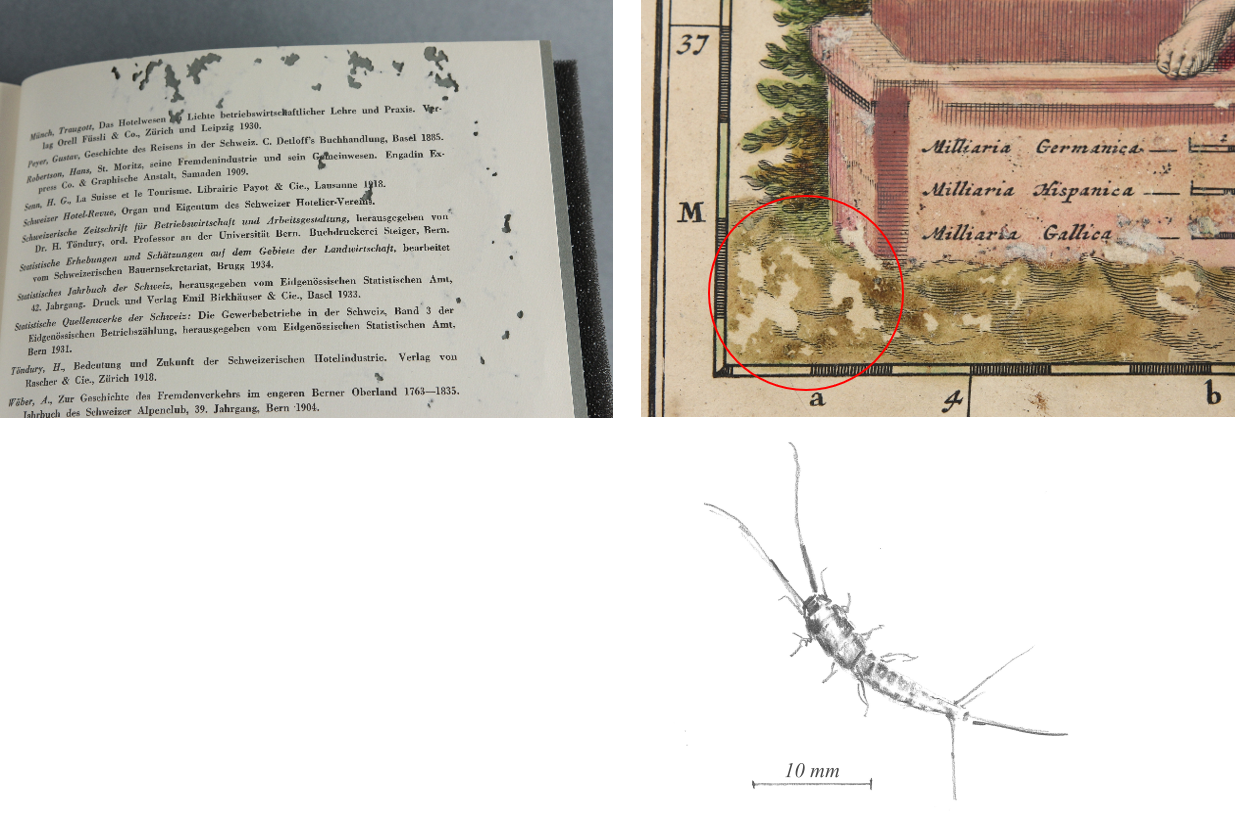
\includegraphics{img/image1.png}
\caption{Typische Frass-Schäden von Silberfischchen
(\emph{lat. lepisma saccharina}) an Büchern und kolorierten Grafiken}
\end{figure}

\begin{figure}
\centering
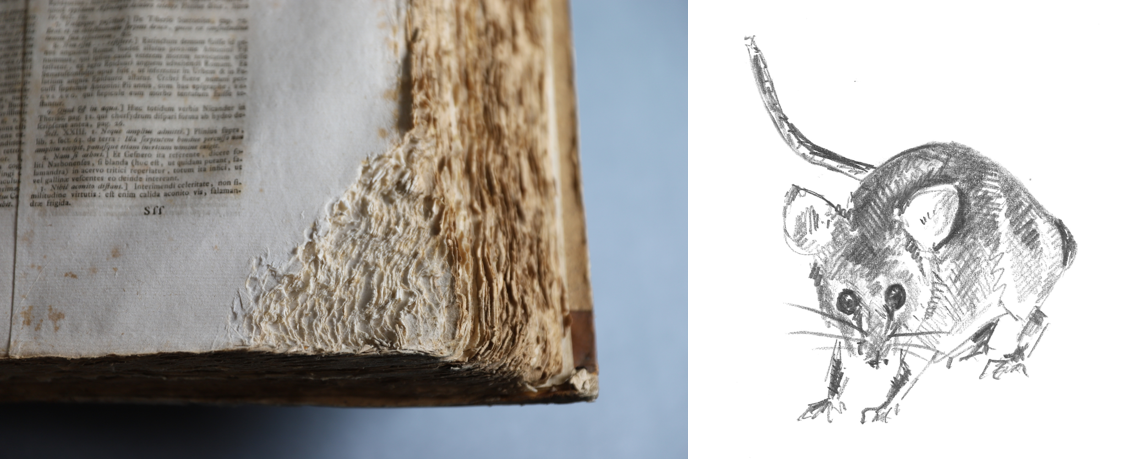
\includegraphics{img/image2.png}
\caption{Frass-Schaden an Buchblock durch Nager}
\end{figure}

Es folgte ein weiterer Auftrag an die Schädlingsbekämpfungsfirma, die
ein Monitoring zuerst jeden zweiten, dann jeden dritten Monat
durchführte. Zwischenzeitlich finden diese noch zweimal im Jahr statt,
aber die Fachleute sind natürlich jederzeit ansprechbar für aktuell
auftauchende Fragen.

Es besteht ein Ess- und Trinkverbot für die Nutzer der Lesesäle und auch
die Mitarbeitenden sind aufgefordert, Essen und Getränke nur an den
dafür vorgesehenen Orten zu konsumieren.

Gleichzeitig haben wir intern in der Dienststelle Konservierung
Ansprechpersonen, welche die Mitarbeitenden in der Bibliothek immer
wieder dazu ermuntern, die Augen offen zu halten und gesichtete Tiere zu
melden, damit sie identifiziert und klassifiziert werden können. Oft
gelangen Insekten von draussen in die Räumlichkeiten, welche
grundsätzlich für unsere Bestände keine Gefahr darstellen. Diese Tiere
sind aber ein gefundenes Fressen für gefährlichere Schädlinge, wenn sie
sich in Ritzen und Ecken verkriechen oder tot als Frass-Köder wirken.
Eine überwachte Klimatisierung der Magazin- und Atelierräumlichkeiten
und die Sicherstellung einer regelmässigen Reinigung sind genauso
wichtig wie das Schädlingsmonitoring. Insekten fühlen sich in Staub und
Schmutz grundsätzlich wohl. Abfälle müssen regelmässig und oft entsorgt
werden.

So sind wir seit dem Wiedereinzug in 2016 von Schädlingsbefall verschont
geblieben und hoffen, dass dies so bleibt. Ein konsequentes Monitoring
ist also weiterhin angezeigt.

Im Rahmen von internen und externen Veranstaltungen finden sporadisch
Weiterbildungen im Restaurierungsatelier statt, dies manchmal auch auf
spielerische Art: Die Teilnehmenden müssen anhand von konkreten
Beispielen an älteren Insekten- und Frass-Schäden herausfinden, welches
Tier hier am Werk war.

\begin{figure}
\centering
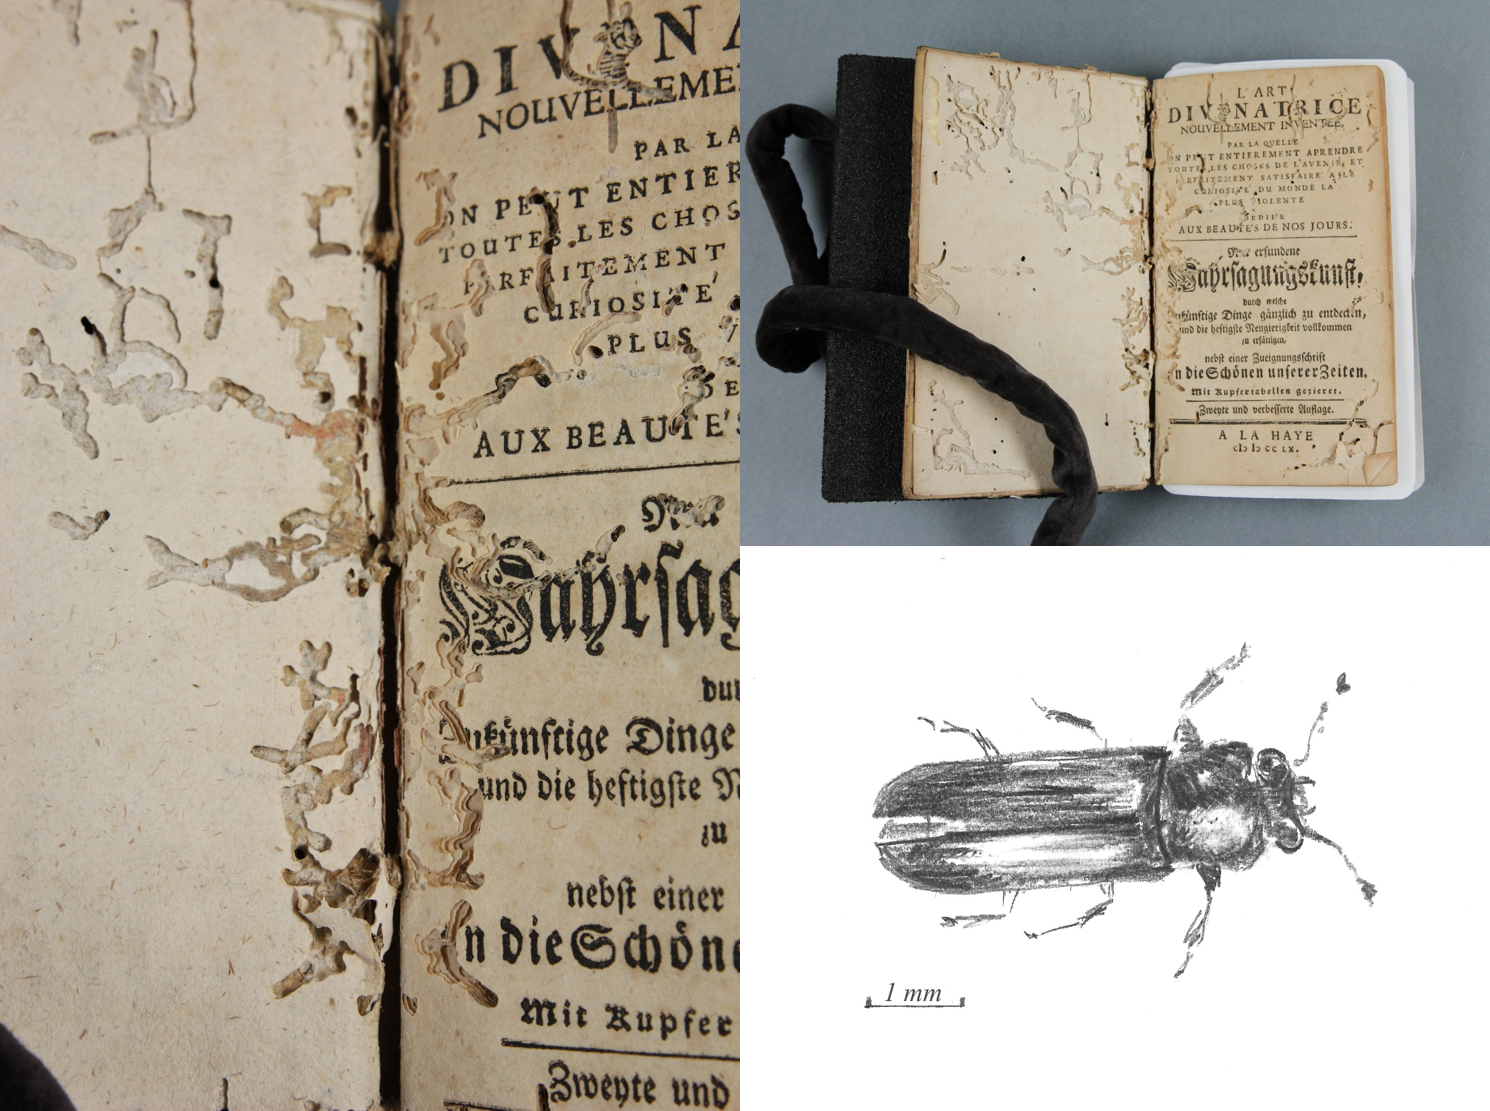
\includegraphics{img/image3.png}
\caption{Frassgänge in Buch durch Larven von Käferarten}
\end{figure}

\hypertarget{hinweis-zum-copyright-der-bilder}{%
\paragraph{Hinweis zum Copyright der
Bilder}\label{hinweis-zum-copyright-der-bilder}}

Fotoaufnahmen: © Zentrum Historische Bestände, Bibliothek Münstergasse
Bern

Zeichnungen: © Andréa E. Bhend, Zentrum Historische Bestände, Bibliothek
Münstergasse Bern

%autor
\begin{center}\rule{0.5\linewidth}{0.5pt}\end{center}

\textbf{Andréa E. Bhend} hat in 1995 in Bern den Abschluss als
Verlagsbuchhändlerin mit Eidg. FA gemacht. Danach arbeitete sie auf dem
erlernten Beruf, führte nebenbei einen eigenen Buchverlag für Lehrmittel
und bildete sich in Werbegrafik \& Design und Webpublishing weiter. Den
Master in Konservierung-Restaurierung an der Hochschule der Künste in
Bern hat sie in 2013 erfolgreich abgeschlossen. Sie ist seit Januar 2014
am Zentrum Historische Bestände als Konservatorin-Restauratorin der
Dienststelle Konservierung an der Bibliothek Münstergasse in Bern tätig
und besucht fachspezifische Weiterbildungen u.a. zum Thema IPM.

Konservatorin-Restauratorin MA Zentrum Historische Bestände Bibliothek
Münstergasse Universitätsbibliothek Bern Münstergasse 61 / Postfach
CH-3000 Bern 8 \url{https://www.unibe.ch} \textbar{}
\href{mailto:andrea.bhend@ub.unibe.ch}{\nolinkurl{andrea.bhend@ub.unibe.ch}}

\end{document}
